\documentclass{standalone}


\usepackage{tikz}
\usetikzlibrary{shapes,backgrounds,calc,patterns}
\usepackage{venndiagram}


\begin{document}
    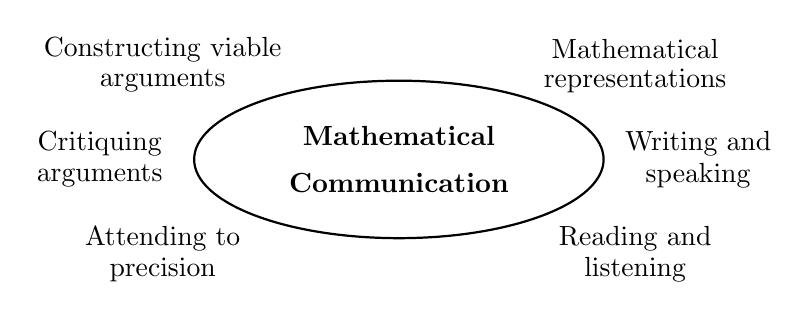
\begin{tikzpicture}
\node at (0,.3) {\textbf{Mathematical}};
\node at (0,-.3) {\textbf{Communication}};
\draw [thick] (0,0) ellipse (2.6 and 1);

\node at (-3,1.4) {Constructing viable};
\node at (-3,1.0) {arguments};

\node at (-3.8,0.2) {Critiquing};
\node at (-3.8,-0.2) {arguments};

\node at (-3,-1.0) {Attending to};
\node at (-3,-1.4) {precision};

\node at (3,1.4) {Mathematical};
\node at (3,1.0) {representations};

\node at (3.8,0.2) {Writing and};
\node at (3.8,-0.2) {speaking};

\node at (3,-1.0) {Reading and};
\node at (3,-1.4) {listening};

\end{tikzpicture}   

\end{document}	